\section{Trabalhos Relacionados} \label{chap:relacionados}

	%O particionamento \hs\ encontra-se em duas principais bordagens sendo essas algoritmos para otimização de escolhas de particionamento e uso de recursos de determinada aplicação e o particionamento para sistemas embutidos.

	%not embedded
	O particionamento de forma geral é um problema de otimização na qual vários autores utilizam métodos para auxiliar na decisão de cada componente do \design\ referencial de \software. Utiliza-se tanto algoritmos exatos quanto heurísticas \cite{Arato2005}.

	\begin{figure}[!b] \centering
    	\vspace{-15pt}
		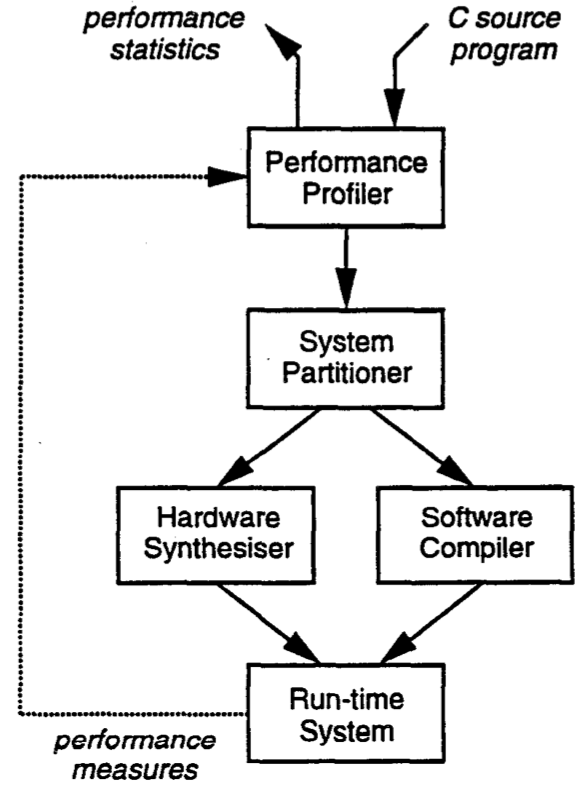
\includegraphics[width=0.21\textwidth]{img/rt-edwards_method.png}
        \vspace{-10pt}
		\caption{Metodologia de \codesign\ de \cite{Edwards1994}. Fonte: \cite{Edwards1994}.}
		\label{fig:tr-edwards_method}
	\end{figure}
	Os autores \cite{Edwards1994} utilizam do particionamento para aprimorar a performance do seu \software. Em seu trabalho, realiza-se a tentativa de tratar regiões críticas da aplicação na qual uma solução em \software\ não pode chegar à restrições de performance requeridas e uma solução em \hardware\ deve ser encontrada, ou a performance total pode ser acelerada pela implementação de uma região crítica em \hardware.
	Em seu trabalho, é apresentada uma metodologia para desenvolvimento \codesign\ no qual consiste na construção do código de uma aplicação em \textit{C} e as regiões críticas são identificadas e particionadas. Feito isso realizar-se mensurações do projeto e uma nova verificação de particionamento é realizada, como é exibido na Figura \ref{fig:tr-edwards_method}.
	Utiliza-se também de um FPGA para as mensuras de performance e a propriedade de reconfiguração para novos testes em \hardware.

	Já o trabalho de \cite{Stitt2003} procura uma abordagem utilizando métodos de otimização de \software\ dinâmicos, introduzindo a primeira abordagem para particionamento de \hs\ dinâmico.
	O processo consiste na deteção da região de \software\ mais frequentemente executada e reimplementa-a em \hardware\ de FPGA.
	Eles afirmam que a utilização de particionamento dinâmico trás uma série de vantagens comparado com abordagens tradicionais.

    Existem vários trabalhos que propuseram algoritmos exatos baseados em \textit{branch-and-Bound} \cite{Jigang2004, Mann2007, Strachacki2008}, programação dinâmica \cite{Madsen1997, Wu2006} e linear inteira (ILP, do inglês \textit{integer linear programming}) \cite{Niemann1997}.

	\cite{Nematbakhsh_theeffect} parte para o exame da relação entre o \textit{footprint} gerado para o FPGA e o \speedup\ do \software\ na situação na qual um FPGA é utilizado para a implementação de \textit{loops} e sub-rotinas críticas.
	Como utilizam uma abordagem direta, utilizaram de ferramentas protótipos e comerciais como \textit{Synopys' Nimble Compiler} e \textit{Proceler}, para a facilitação do processo.

	Abordagens mais recentes como a de \cite{Yan2017} usa o método de particionamento \hs baseado em otimização \textit{position disturbed particle swarm} com otimização invasiva de \textit{weed}.

	\cite{Wang2016} citam que o particionamento depende da exploração de caracterização, estimação e \design\ espacial das métricas de custo e performance sistêmica. É exaltado também que o \codesign\ nos dias de hoje é tão complexo que a simplificação do particionamento só para duas partes não é suficiente para a representação do problema como um todo. Sobre essa crítica, dissertam sobre a inclusão de parâmetros chave de \design\ e uso de recursos que deveriam ser incorporados à modelagem do sistema e dessa forma, o trabalho proposto por eles visa considerar a modelagem de incerteza para particionamento de sistemas com um conjunto melhorado de parâmetros para compartilhamento de recursos \hs.
	Esse terceiro item a ser considerado ao problema de particionamento podem ser definidos em três tipos sendo essas: \textit{a)} o conjunto de recursos necessários para particionar uma dada tarefa (sendo esses RAM, ROM, DPS, blocos IP do inglês, \textit{intelectual propriety}, entre outros); \textit{b)} tarefaz que possuem vários parâmetros de configurações que provê diferentes \textit{trade-off} entre recursos e performances como por exemplo circuitos de multiplicações/divisões que podem ser sintetizados sequencialmente (pouca área e lento) ou combinatório\footnote{Por \textit{unrolling}, técnica de otimização de código no qual tenta reduzir ou eliminar as iterações de determinado \textit{loop} do código.} (muita área e rápido); \textit{c)} a dificuldade da mensura de desempenho e impacto no uso de recursos em várias configurações de partição com precisão precisando ter em mente a partição com a natureza incerta dessas estimativas não precisas.
	A teoria da incerteza é uma abordagem que é um sistema matemático que é designado para modelar indeterminância ao invés do uso da teoria da probabilidade. Isso pois, quanto tem-se muitas amostras de uma quantidade indeterminada, seria significativo a utilização da teoria de probabilidade ou \textit{fuzzy} pela propriedade de serem contínuas entre o intervalo 0 (zero) à 1 (um). Entretanto, se não possui-se amostras suficientes para a estimação de uma distribuição de probabilidade, utiliza-se do conhecimento do domínio para avaliação do grau de crença de que cada evento indeterminado acontecerá, no caso, aplicado pela teoria da incerteza. A teoria da incerteza é um ramo da matemática axiomática para modelagem de graus de crença, de modo geral.

	Como outro trabalho recente que aborda o particionamento, \cite{Choi2016} descreve um \textit{framework} chamado LegUp.
	Com essa ferramenta é possível compilar um \software\ e suas \textit{threads} gerando um sistema \textit{hardware-only} ou também um sistema híbrido particionado paralelo utilizando aceleradores, gerando também todos os itens necessários para tal como memórias sintetizadas e sistemas de interconexões. Utilizam duas técnicas de descrição de paralelismo em \software\ sendo elas a \textit{Pthreads} e a \textit{OpenMP} sendo a primeira permite a sintetização de funções operando concorrentemente em \hardware\ com aceleradores, e a segunda usada para gerar os próprios aceleradores executados concorrentemente em um sistema de compartilhamento de memória.
	Afirmam também que a sua ferramenta produz HDL de alta performance que pode ser comparado com circuitos que são gerados por ferramentas HLS comerciais.

	Entretanto, além de todo arcabouço de algoritmos para escolhas para sistemas de propósito geral tal como os citados, existe uma subconjunto específico do problema na qual trata-se do particionamento em sistemas embutidos.


	% Embedded
	O desenvolvimento para sistemas \hs\ participativo para sistemas embutidos ou microcontroladores já é pesquisado amplamente como os trabalhos de \cite{Ernst1993, Gupta1995, Hardt1995, Gajski1994, Bolsens1997}, publicados na década de 90.
	\cite{Mei2000} em seu trabalho, descreve um particionamento de \hs\ além de uma abordagem de escalonamento para sistemas embutidos dinamicamente reconfiguráveis (DRESs, do inglês \textit{dynamically reconfigurable embedded systems}) no qual possuem como projeto um processador de propósito geral junto com um FPGA sendo este reconfigurável em tempo de execução para reduzir custos. Dessa forma, seu trabalho consiste numa análise de tempo de configuração e, como contribuição, a análise do tempo de reconfiguração parcial do FPGA.
	%Com a adição da reconfiguração parcial de \hardware, o escalonamento no FPGA torna-se um problema de alocação restrita, enquanto o escalonamento em circuitos integrados de aplicação específica (ASICs, do inglês \textit{application-specific integrated circuits}) é um problema de serialização.
	Para o escalonamento, \cite{Mei2000} utiliza um método baseado na heurística do algoritmo genético (GA, do inglês \textit{genetic algorithm}) e num algoritmo de escalonamento de lista com melhorias.
	O escalonador desenvolvido atua como uma sub-rotina do algoritmo de particionamento. Ele é invocado no passo \textit{evolution} do GA. Além do escalonamento já conhecido em processador e barramento sequenciais determinando a ordem e tempo início de execução, o algoritmo também deve fazer o escalonamento no FPGA. Mas não só determinando o tempo de início da tarefa, mas sim sua posição no FPGA respeitando as restrições de recursos e precedentes, tornando assim o problema uma abordagem ao problema de alocação restrita.

	Já \cite{Arato2003} descreve algumas versões diferentes do problema de particionamento, correspondendo à sistemas de tempo-real e custo restringido, respectivamente fornecendo análise matemática formal para o problema, provando que são problemas $ \mathcal{NP} $-difícil no caso geral. Apresentaram uma abordagem baseada na programação linear inteira resolvendo o problema de forma otimizada, mesmo para sistemas de grande porte, além de outra abordagem utilizando a heurística GA na qual encontrar soluções próximas ao ótimo para sistemas largos.

	\cite{Mann2007}, em \cite{Mann2007}, descreveram uma primeira tentativa para um algoritmo exato, não heurístico, para o problema de particionamento. Eles utilizam um esquema na qual utilizam a estratégia \textit{branch-and-bound} como um \textit{framework}, permitindo o incremento de outros algoritmos. Em sua implementação, realizaram várias investigações para incrementar a eficiência do algoritmo, incluindo várias técnicas sendo elas: \textit{lower bounds based on LP-relaxation}, uma mecânica de inferência customizada, condições não-triviais necessárias baseadas num algoritmo \textit{minimum-cut}, e diferentes heurísticas com passos pré-otimizados. O algoritmo também pode ser generalizado a fim de incluir mais de uma restrição, podendo também o \designer\ prescreva quais nós devem estar em qual nível de projeto. Eles demonstram que o produto pode resolver problemas de particionamento altamente complexos em tempo razoável. Citam que é cerca de dez minutos mais rápido que algoritmos exatos anteriores baseados em programação linear inteira para os testes realizados.

	Pesquisas mais recentes como a de \cite{Hassine2017}, em \cite{Hassine2017}, procuravam aplicar otimizações sobre o tempo de execução e gasto energético para \cores\ baseados em sistemas embarcados por meio de algoritmos de particionamento.
	O algoritmo proposto é destina-se a alcançar um particionamento de grafos à procurar o melhor conjunto da relação energia e tempo de execução.
	Testado em comparação com outros algoritmos heurísticos como \textit{Simulated Annealing}, Busca Tabu e Genético, o algoritmo mostra-se ser melhor adequado para aplicações em \cores\ baseados em sistemas embarcados que necessitam do equilíbrio no \textit{tradeoff} de sistemas embarcados.

	\cite{Trindade2016} por exemplo utiliza do GA para solucionar o problema de particionamento em sistemas embutidos. Em seu trabalho, é proposto novas abordagens para o problema usando técnicas de verificação baseadas nas teorias de módulo de satisfação (SMT, do inglês \textit{satisfiability modulo theories}). Apresentam um exemplo de particionamento, modelam e solucionam-o usando três diferentes técnicas sendo a principal ideia é aplicar mo método de verificação SMT ao particionamento \hs, e por fim, comparar os resultados com técnicas de otimizações tradicionais como ILP e GA.

	\cite{Jozwiak2017} em seu \textit{survey} publicado em \cite{Jozwiak2017}, considera vários aspectos de uma aplicação embutida, bem como suas tecnologias de \design\ com foco sistemas móveis modernos e \wearables.
	É citado dois paradigmas de desenvolvimento para sistemas embutidos sobre sistema de multi-processadores heterogêneos sendo eles o paradigma de sistemas \textit{life-inspired} e sistemas \textit{quality-driven}. O paradigma de sisetmas \textit{life-inspired} especifica princípios básicos, características e organização funcional e estrutural de um sistema embutido por meio da analogia à vida de um organismo inteligente, além de básicas soluções de mecanismos e arquiteturas de sistemas para implementar tais princípios. Já o paradigma de sistemas \textit{quality-driven} (ou seja, orientado pela qualidade) torna-se uma segunda solução para o \design\ de dispositivos que necessitam satisfazer as exisgências de \textit{real-time}, baixo consumo de energia, entre outros. Dessa forma, especifica-se qual a nova qualidade do sistema a ser requeria e como esta meta é obtida. De forma a facilitar a compreensão, \cite{Jozwiak2017} define qualidade de uma solução sistemica proposto como o total de sua eficácia e eficiência na resolução do problema real. Eficácia entende-se como o grau em que uma solução atinge seus objetivos e a eficiência o grau em que uma solução usa recursos para realizar seus objetivos e juntas determinam o grau de excelência. Elas são expressas em termos de parâmetros mensuráveis, o que é necessário para implementar o design \textit{quality-driven}. Entretanto, é descrito ao final que, enquanto \designers\ aprenderam bastante na construção de plataformas de \hardware\ heterogêneos altamente paralelos, os métodos e ferramentas automatizadas para a sua programação e o paralelismo do algoritmo, bem como o \codesign\ coerente da arquitetura \hs\ ainda são atrasados perante à tecnologia.
	Por fim, o \textit{survey} não menciona nenhuma pesquisa feita sobre particionamento para sistemas \wearables.
